\documentclass[12pt, a4paper, oneside]{ctexart}
\usepackage{amsmath, amsthm, amssymb, bm, color, graphicx, geometry, mathrsfs,extarrows, braket, booktabs, array, xcolor, fontspec, appendix, float, subfigure, wrapfig, enumitem}
\usepackage[colorlinks,linkcolor=red,anchorcolor=blue,citecolor=blue,urlcolor=blue,menucolor=black]{hyperref}

%%%% 设置中文字体 %%%%
\setCJKmainfont{方正新书宋_GBK.ttf}[BoldFont = 方正小标宋_GBK, ItalicFont = 方正楷体_GBK, BoldItalicFont = 方正粗楷简体]
%%%% 设置英文字体 %%%%
\setmainfont{Times New Roman}
\setsansfont{Calibri}
\setmonofont{Consolas}

%%%% 设置代码块 %%%%
% 在vscode中使用minted需要先配置python解释器, Ctrl+Shift+P, 输入Python: Select Interpreter选择安装了Pygments的Python版本. 再在setting.json中xelatex和pdflatex的参数中加入 "--shell-escape", 即可
% TeXworks中配置方法参考: https://blog.csdn.net/RobertChenGuangzhi/article/details/108140093
\usepackage{minted}
\renewcommand{\theFancyVerbLine}{
    \sffamily\textcolor[rgb]{0.5,0.5,0.5}{\scriptsize\arabic{FancyVerbLine}}} % 修改代码前序号大小
% 加入不同语言的代码块
\newmintinline{cpp}{fontsize=\small, linenos, breaklines, frame=lines}
\newminted{cpp}{fontsize=\small, linenos, breaklines, frame=lines}
\newmintedfile{cpp}{fontsize=\small, linenos, breaklines, frame=lines}
\newmintinline{matlab}{fontsize=\small, linenos, breaklines, frame=lines}
\newminted{matlab}{fontsize=\small, mathescape, linenos, breaklines, frame=lines}
\newmintedfile{matlab}{fontsize=\small, linenos, breaklines, frame=lines}
\newmintinline{python}{fontsize=\small, linenos, breaklines, frame=lines, python3}  % 使用\pythoninline{代码}
\newminted{python}{fontsize=\small, linenos, breaklines, frame=lines, python3}  % 使用\begin{pythoncode}代码\end{pythoncode}
\newmintedfile{python}{fontsize=\small, linenos, breaklines, frame=lines, python3}  % 使用\pythonfile{代码地址}

%%%% 设置行间距与页边距 %%%%
\linespread{1.2}
\geometry{left=2.5cm, right=2.5cm, top=2.5cm, bottom=2.5cm}

%%%% 定理类环境的定义 %%%%
\newtheorem{example}{例}            % 整体编号
\newtheorem{theorem}{定理}[section] % 定理按section编号
\newtheorem{definition}{定义}
\newtheorem{axiom}{公理}
\newtheorem{property}{性质}
\newtheorem{proposition}{命题}
\newtheorem{lemma}{引理}
\newtheorem{corollary}{推论}
\newtheorem{condition}{条件}
\newtheorem{conclusion}{结论}
\newtheorem{assumption}{假设}
\numberwithin{equation}{section}  % 公式按section编号 (公式右端的小括号)
\newtheorem{algorithm}{算法}

%%%% 自定义环境 %%%%
\newsavebox{\nameinfo}
\newenvironment{myTitle}[1]{
    \begin{center}
    {\zihao{-2}\bf #1\\}
    \zihao{-4}\it
}{\end{center}}  % \begin{myTitle}{标题内容}作者信息\end{myTitle}
\newcounter{problem}  % 问题序号计数器
\newenvironment{problem}[1][]{\stepcounter{problem}\par\noindent\textbf{题目\arabic{problem}. #1}}{\smallskip\par}
\newenvironment{solution}[1][]{\par\noindent\textbf{#1解答. }}{\smallskip\par}  % 可带一个参数表示题号\begin{solution}{题号}
\newenvironment{note}{\par\noindent\textbf{注记. }}{\smallskip\par}
\newenvironment{remark}{\begin{enumerate}[label=\textbf{注\arabic*.}]}{\end{enumerate}}
\BeforeBeginEnvironment{minted}{\vspace{-0.5cm}}  % 缩小minted环境距上文间距
\AfterEndEnvironment{minted}{\vspace{-0.2cm}}  % 缩小minted环境距下文间距

%%%% 图片相对路径 %%%%
\graphicspath{{figure/}} % 当前目录下的figure文件夹, {../figure/}则是父目录的figure文件夹
\setlength{\abovecaptionskip}{-0.2cm}  % 缩紧图片标题与图片之间的距离
\setlength{\belowcaptionskip}{0pt} 

%%%% 缩小item,enumerate,description两行间间距 %%%%
\setenumerate[1]{itemsep=0pt,partopsep=0pt,parsep=\parskip,topsep=5pt}
\setitemize[1]{itemsep=0pt,partopsep=0pt,parsep=\parskip,topsep=5pt}
\setdescription{itemsep=0pt,partopsep=0pt,parsep=\parskip,topsep=5pt}

%%%% 自定义公式 %%%%
\everymath{\displaystyle} % 默认全部行间公式, 想要变回行内公式使用\textstyle
\DeclareMathOperator*\uplim{\overline{lim}}     % 定义上极限 \uplim_{}
\DeclareMathOperator*\lowlim{\underline{lim}}   % 定义下极限 \lowlim_{}
\DeclareMathOperator*{\argmax}{arg\,max}  % 定义取最大值的参数 \argmax_{}
\DeclareMathOperator*{\argmin}{arg\,min}  % 定义取最小值的参数 \argmin_{}
\let\leq=\leqslant % 简写小于等于\leq (将全部leq变为leqslant)
\let\geq=\geqslant % 简写大于等于\geq (将全部geq变为geqslant)
\DeclareRobustCommand{\rchi}{{\mathpalette\irchi\relax}}
\newcommand{\irchi}[2]{\raisebox{\depth}{$#1\chi$}} % 使用\rchi将\chi居中

%%%% 一些宏定义 %%%%
\def\bd{\boldsymbol}        % 加粗(向量) boldsymbol
\def\disp{\displaystyle}    % 使用行间公式 displaystyle(默认)
\def\tsty{\textstyle}       % 使用行内公式 textstyle
\def\sign{\text{sign}}      % sign function
\def\wtd{\widetilde}        % 宽波浪线 widetilde
\def\R{\mathbb{R}}          % Real number
\def\N{\mathbb{N}}          % Natural number
\def\Z{\mathbb{Z}}          % Integer number
\def\Q{\mathbb{Q}}          % Rational number
\def\C{\mathbb{C}}          % Complex number
\def\K{\mathbb{K}}          % Number Field
\def\P{\mathbb{P}}          % Polynomial
\def\d{\mathrm{d}}          % differential operator
\def\e{\mathrm{e}}          % Euler's number
\def\i{\mathrm{i}}          % imaginary number
\def\re{\mathrm{Re}}        % Real part
\def\im{\mathrm{Im}}        % Imaginary part
\def\res{\mathrm{Res}}      % Residue
\def\ker{\mathrm{Ker}}      % Kernel
\def\vspan{\mathrm{vspan}}  % Span  \span与latex内核代码冲突改为\vspan
\def\O{\mathcal{O}}          % Polynomial
\def\L{\mathcal{L}}         % Loss function
\def\wdh{\widehat}          % 宽帽子 widehat
\def\ol{\overline}          % 上横线 overline
\def\ul{\underline}         % 下横线 underline
\def\add{\vspace{1ex}}      % 增加行间距
\def\del{\vspace{-1.5ex}}   % 减少行间距

%%%% 正文开始 %%%%
\begin{document}
\begin{myTitle}{算法设计与分析-上机实验作业}
    吴天阳\ 2204210460\ 强基数学002
\end{myTitle}
\section{问题一}
给定由$n$个数组成的集合$S$,从中找出与$S$的中位数最近的$n/4$个元素,请设计一个最坏情况下时间复杂度为$\O(n)$的算法.
\subsection{问题分析}
首先要实现\textbf{线性时间选择}代码,即\cppinline{select(l, r, k)}函数,在$\O(n)$时间复杂度下找到数组\cppinline{a[l,...,r]}中第$k$大的数字. 当$k = \lfloor(n+1)/2\rfloor$时就是查找中位数.

\subsubsection{randomizedSelect方法}
考虑快排的思路,我们考虑划分函数\cppinline{partition(l,r)}对数组\cppinline{a[l,...,r]}进行划分:随机选取一个元素\cppinline{a[i]}作为基准元素,然后将\cppinline{a[l,...,r]}中小于等于\cppinline{a[i]}的元素移动到左侧,大于等于\cppinline{a[i]}的元素移动到右侧,通过该方法,可以得到小于等于\cppinline{a[i]}的元素个数记为$m$.

假设当前查询的第$k$大的数字,如果$k\leq m$则在\cppinline{a[l,...,m]}中继续查找第$k$大的元素,否则在\cppinline{a[m+1,...,r]}中查找第$k-m$大的元素,该操作可以递归完成.

该时间复杂度平均为$\O(n)$,但是如果每次选取的最小的元素作为基准,而我们查询的是最大的元素,则时间复杂度最差可能达到$\O(n^2)$,于是我们需要对其进行改进.
\subsubsection{select方法}
在\cppinline{randomizedSelect}方法的基础上,我们发现由于每次是随机选取的一个基准,该基准可能较差(过于偏向左侧或右侧),所以我们期望选择一个较为靠中间的元素,这样就能保证每次必定减少$n$的某一个量级,从而稳定最坏复杂度.

假设当前处理的序列长度为$n$,序列为\cppinline{a[1,...,n]},具体思想就是找当前序列的\textbf{中位数的中位数}作为基准.

具体做法:我们假设以$5$个元素作为一个小组,将原数组划分为$\lfloor n/5\rfloor$个模$5$的剩余类,例如$n=17$,则划分后的结果为\cppinline{[*****|*****|*****|**]}(\cppinline{*}表示数组中的元素,一共得到$3$个小组),然后我们对每个小组中的元素使用冒泡排序,冒泡$3$次即可找到小组中的中位数,我们将中位数标记为\cppinline{$}符号,则排序后数组为\cppinline{[**$**|**$**|**$**|**]}. 然后我们将每个小组的中位数全部移动到整个数组的左侧,即\cppinline{[$$$**|*****|*****|**]},于是我们已经获得了中位数序列,即数组中开头三个,为了求解中位数的中位数,我们再递归调用\cppinline{select}函数. 以上面例子为例,我们只需求解\cppinline{select(1,3,2)}从而求解\cppinline{[$$$]}中的中位数,即可得到原数组的中位数的中位数.

获得中位数的中位数\cppinline{x}后,再以\cppinline{x}作为基准元素,利用类似快排的划分函数\\\cppinline{partition(l,r,x)}(只不过这次给定了基准元素\cppinline{x}),从而对原数组左右划分,再判断我们要查询的第$k$大元素是在基准的左侧还是右侧,递归查找即可.

\textbf{注}:如果有存在多个重复基准元素\cppinline{x},我们需要将划分后的\textbf{基准元素全部聚集在中间},假设有$m$个重复基准元素,于是原数组最终应该划分为\cppinline{[00000|$$$$|11111]},其中\cppinline{0}、\cppinline{1}分别表示小于、大于基准元素的值,\cppinline{$}表示基准元素. 于是原数组被划分为三分,如果当前第$k$大元素落在中间的区间中,则直接返回基准元素,否则判断第$k$大元素在左侧还是右侧,递归查找即可.

上述算法那的关键就是找到了当前序列的中位数的中位数,从而每次划分为两半时,基准元素左侧至少会有$\lfloor n/4\rfloor$个元素. 保证每次查找至少可以减少$\lfloor n/4\rfloor$的数量级.

理论复杂度分析,设对序列长度为$n$的序列调用\cppinline{select}函数需要$T(n)$的时间,则查找中位数的中位数至多使用$T(n/5)$,使用基准$x$划分原数组,两个数组中至多还有$3n/4$个元素,则进一步递归调用至多使用$T(3n/4)$时间. 综上,$T(n)$递推式为
\begin{equation*}
    T(n) = Cn+T(n/5)+T(3n/4),\ (C\approx 3)
\end{equation*}
常数$C$主要包含每个小组的冒泡排序、\cppinline{partition}、聚集基准元素所花的时间.
\subsubsection{查找距离中位数最近的k个数}
有了\cppinline{select}函数,这个问题就非常容易解决了,首先找到原数组的中位数\cppinline{mid},然后求原数组与\cppinline{mid}的绝对值之差,存为数组\cppinline{b[]},然后查找数组\cppinline{b[]}的第$k$大元素\cppinline{delta},那么说明和\cppinline{mid}相差\cppinline{delta}距离的元素就是距离中位数\cppinline{mid}最近的$k$个元素,最后搜索一遍原数组,将满足$|a[i] - mid|\leq delta$的元素输出出来即可.
\subsection{算法实现}
\begin{cppcode}
const int N = 1e8;

int n, k, a[N], b[N], tmp[N];

void bubble(int l, int r) {  // 对a[l,r)进行冒泡排序
    for (int i = l; i < r; i++)
        for (int j = i + 1; j < r; j++)
            if (a[i] > a[j]) swap(a[i], a[j]);
}
// 划分函数,返回值为:最靠左的mid下标,与mid相同数个数
pair<int, int> partition(int l, int r, int mid) {
    int i = l - 1, j = r;
    while (1) {
        while (a[++i] < mid && i < r);
        while (a[--j] > mid && j >= l);
        if (i >= j) break;
        swap(a[i], a[j]);
    }
    // 例mid=5, [0 3 2 5 5 5 5 14 12 11], ll=2, rr=7
    int ll = j, rr = j+1;  // 与mid相同数合并称一块
    for (int i = 0; i < ll; i++) {
        while (a[ll] == mid && ll > l) ll--;
        if (a[i] == mid) swap(a[i], a[ll]), ll--;
    }
    for (int i = r-1; i > rr; i--) {
        while (a[rr] == mid && rr < r-1) rr++;
        if (a[i] == mid) swap(a[i], a[rr]), rr++;
    }
    return make_pair(ll+1, rr-ll-1);
}

int select(int l, int r, int k) {  // 返回a[l,r)中第k大的元素
    if (r - l < 5) { // 如果元素个数小于5
        bubble(l, r);
        return a[l+k-1];
    }
    // [00000|00000|00000|000]  以五个进行一个划分,每个子区间长度为5
    for (int i = 0; i < (r - l) / 5; i++) {
        int s = l + 5 * i, t = s + 5;  // 处理子区间[s,t)
        for (int j = s; j < s+3; j++)  // 仅需做3次冒泡
            for (int k = j+1; k < t; k++)
                if (a[j] > a[k]) swap(a[j], a[k]);
        swap(a[l+i], a[s+2]);  // 将[s,t)的中位数移动到数列开头
    }
    int x = select(l, l+(r-l)/5, (r-l+5)/10);  // 递归找到中位数的中位数
    auto p = partition(l, r, x);
    int mid = p.first, same = p.second, less = mid-l;  // 以mid作为快排基准进行排序
    if (k <= less) return select(l, mid, k);  // 在左半区间
    else if (k <= less + same) return x;  // 在中间区间就是中位数
    return select(mid+same, r, k-less-same);  // 在右半区间
}

int main() {  // 求解距离中位数n/4近的数
    cin >> n;
    for (int i = 0; i < n; i++) cin >> a[i];
    memcpy(tmp, a, sizeof(int) * n);
    int mid = select(0, n, (n+1)/2);  // 先求出中位数
    cout << "mid: " << mid << '\n';
    for (int i = 0; i < n; i++) a[i] = abs(a[i] - mid);  // 求出绝对值数组
    int k = select(0, n, n/4), tot = n/4;  // 绝对值数组中前n/4分位数
    memcpy(a, tmp, sizeof(int) * n);
    cout << "Around Mid: ";
    for (int i = 0; i < n && tot; i++)  // 再从原数组中找绝对值差小于等于k的
        if (abs(a[i] - mid) <= k) {
            cout << a[i] << ' ';
            tot--;
        }
    cout << '\n';

    // 将原数组排序,检查结果是否正确
    cout << "\n" << "After sorted(Check): " << '\n';
    sort(a, a + n);
    for (int i = 0; i < n; i++)
        cout << a[i] << ' ';
    cout << '\n';
    return 0;
}
\end{cppcode}
\subsection{测试结果与性能分析}
测试结果(两个测试数据\cppinline{Input}为输入数据,\cppinline{Output}为输出结果,\cppinline{mid}为中位数,\cppinline{Around Mid}为中位数最近的$n/4$个值):
\begin{cppcode}
Input:
9
1 2 2 3 4 5 5 8 9
Output:
mid: 4
Around Mid: 3 4

Input:
20
34 26 98 31 26 88 90 39 68 95 80 78 69 7 3 48 32 39 9 63 
Output:
mid: 39
Around Mid: 34 31 39 32 39
\end{cppcode}
为了和直接排序的速度进行比较,我分别构造了$n=10^7$和$n=10^8$的序列长度,然后分别利用\cppinline{select}函数和直接排序输出第$k$大元素速度进行了比较,代码如下
\begin{cppcode}
int main() {  // 用于测试select函数速度
    ios::sync_with_stdio(0);
    cin.tie(0);
    freopen("in.in", "r", stdin);  // 数据读入
    cin >> n;
    for (int i = 0; i < n; i++) cin >> a[i];
    clock_t start = clock();
    cout << "My Answer: " << select(0, n, 10) << '\n';
    clock_t end = clock();
    cout << "Use Time: " << end - start << "ms" << '\n';
    
    int *tmp = new int[sizeof(a)/sizeof(int)];
    memcpy(tmp, a, sizeof(a));
    start = clock();
    sort(a, a + n);
    cout << "Check: " << a[10-1] << '\n';
    end = clock();
    cout << "Use Time: " << end - start << "ms";
    return 0;
}
\end{cppcode}
测速速度结果为:

$n=10^7$结果\cppinline{select}函数$697$ms,直接排序所用时间$1481$ms.

$n=10^8$结果\cppinline{select}函数$5866$ms,直接排序所用时间$12523$ms.

可以看出来\cppinline{select}函数快了一倍左右,效果不错.
\subsection{数据生成代码}
\begin{cppcode}
#include <iostream>
#include <time.h>
using namespace std;

int main() {  // 7-1随机生成数据
    srand(time(NULL));  // 随机种子
    freopen("7-1.in", "w", stdout);  // 输出文件到"7-1.in"中
    int n = 1e7;  // 序列总长度
    cout << n << '\n';
    for (int i = 0; i < n; i++) {
        printf("%d ", rand() % 100);
    }
    cout << '\n';
    return 0;
} 
\end{cppcode}
\clearpage
\section{问题二}
设\cppinline{A[1..M], B[1..N],C[1..L]}是三个任意序列,A、B、C的公共超序列定义为一个包含A、B、C为子序列的序列. 请设计实现一个动态规划算法,找出A、B、C的最短公共超序列.
\subsection{问题分析}
\subsubsection{二维最短共超序列}
考虑两个序列\cppinline{a[1,...,n],b[1,...,m]}的最短共超序列,设二维动态规划数组\cppinline{dp[i][j]}表示\cppinline{a[1,...,i]}和\cppinline{b[1,...,j]}的最短共超序列长度,有如下状态转移方程:
\begin{equation*}
    dp[i,j]=\begin{cases}
        dp[i-1,j-1]+1,&\quad a[i] = b[j],\\
        \min\bigg\{dp[i,j-1], dp[i-1,j]\bigg\}+1,&\quad a[i]\neq b[j].
    \end{cases}
\end{equation*}
初始化:$dp[i,0] = i,\ (i=1,2,\cdots, n), dp[0,j] = j,\ (j=1,2,\cdots, m)$.\\
设计思路:若$a[i]=a[j]$,则\cppinline{(i,j)}的最短共超序列可以在\cppinline{(i-1,j-1)}的最短共超序列基础上加上\cppinline{a[i]};若$a[i]\neq a[j]$,则从\cppinline{(i-1,j)}的最短共超序列基础上加上\cppinline{a[i]},也可以从\cppinline{(i,j-1)}的最短共超序列基础上加上\cppinline{b[j]}得到,所以取\cppinline{dp[i][j-1],dp[i-1][j]}中较小者进行转移得到.

生成最短共超序列的方法:通过数组\cppinline{fa[i][j]}记录每次\cppinline{dp[i][j]}的转移来自于谁,于是也可以得到每次需要加上哪一个元素. 例如:记\cppinline{fa=0,1,2}分别表示从\cppinline{dp[i-1][j-1], dp[i-1][j], dp[i][j-1]}转移得到的,那么对应增加的元素分别是\cppinline{a[i], a[i], b[j]}(第一个也可以是\cppinline{b[i]},因为两者相同).

然后从\cppinline{dp[n][m]}开始逆推,逆推方向是\cppinline{dp[i][j]}转移方向,还有\cppinline{(i,j)}处需增加的元素,两者均可通过\cppinline{fa[i][j]}的取值得到.

二维最短共超序列求解可以参考 \href{https://blog.csdn.net/qq_43610614/article/details/107826054}{CSDN - 最短公共超序列(最短公共父序列)}.
\subsubsection{三维最短共超序列}
有了二维的最短共超序列求解办法,我们进一步讨论三维最短共超序列的求解问题. 考虑三个序列\cppinline{a[1,...,n], b[1,...,m], c[1,...,l]}的最短共超序列. 设三维动态规划数组\cppinline{dp[i][j][k]}表示\cppinline{a[1,...,i],b[1,...,m],c[1,...,l]}的最短共超序列,有如下状态转移方程:
\begin{equation*}
    dp[i,j,k]=\begin{cases}
        dp[i-1,j-1,k-1]+1,&\quad a[i]=b[j]=c[k],\\
        dp[i-1,j-1,k]+1,&\quad a[i]=b[j],\\
        dp[i-1,j,k-1]+1,&\quad a[i]=c[k],\\
        dp[i,j-1,k-1]+1,&\quad b[j]=c[k],\\
        \min\bigg\{dp[i-1,j,k],dp[i,j-1,k],dp[i,j,k-1]\bigg\}+1&\quad \text{否则}.
    \end{cases}
\end{equation*}
初始化:$dp[i,j,0],dp[i,0,k],dp[0,j,k],\ (i\in[1,n], j\in[1,m], k\in[1,l])$分别是二维最短共超序列的解,也就是说$dp[i,j,0]= dp'[i,j]$,$dp'[i,j]$是\cppinline{a[1,...,i],b[1,...,j]}的最短共超序列的解. (\textbf{2.1.1}中所介绍的方法求解)

三维最短共超序列的状态转移方程设计思路与二维完全一致,这里不详细解释,反向求解最优解过程也完全一致,只是把二维问题换为三维,\cppinline{fa}数组的取值变为$7$个.

\subsubsection{不能将三维问题转化为两个二维问题求解}
这里说明不能通过分别求解数组\cppinline{a,b}的最短共超序列\cppinline{d},再求解\cppinline{d,c}的最短共超序列,从而得到\cppinline{a,b,c}的最短共超序列.

反例:设\cppinline{a="abed", b="ecaa", c="eacd"},则\cppinline{d="abedcaa"},于是得到错误的最短共超序列为\cppinline{"abedcaacd"},长度为$9$;而最优解应该为\cppinline{"ecabeacd"},长度为$8$.
\subsection{算法分析}
主要是设计如何在三维数组中计算二维的最短共超序列,记少掉的维度为\cppinline{dim},由于二维中\cppinline{fa}数组只有$3$种取值,而三维中有$7$中取值,所以降到二维后还需将\cppinline{fa}数组进行对应,记为\cppinline{idx[3]}. 于是就有了下述代码中$12$到$23$行的内容.
\begin{cppcode}
#include <iostream>
#include <string.h>
#include <algorithm>
using namespace std;
const int N = 310;
char s[3][N];  // 初始字符串
int dp[N][N][N], fa[N][N][N]; // fa={0,...,6}分别表示7个转移方向,具体方向如下面所定义
int dx[7] = {-1, -1, -1, 0, -1, 0, 0};
int dy[7] = {-1, -1, 0, -1, 0, -1, 0};
int dz[7] = {-1, 0, -1, -1, 0, 0, -1};

// dim为排除的维数,idx[0,1,2]分别为返回a-1,b-1;a-1;b-1的转移方向编号
int dim, idx[3];
// 返回a数组在排除dim维度后的i,j对应指针
int* get_prt(int a[][N][N], int i, int j) {
    if (dim == 0) return &a[0][i][j];
    else if (dim == 1) return &a[i][0][j];
    return &a[i][j][0];
}
// 返回数组a在排除dim维度后的i,j元素值
int get(int a[][N][N], int i, int j) {return *get_prt(a, i, j);}
// 设置数组a在排除dim维度后的i,j元素值
void set(int a[][N][N], int i, int j, int x) {*get_prt(a, i, j) = x;}

// 处理a,b的最短共超序列
void subsolve(char a[], char b[]) {
    int l1 = strlen(a+1), l2 = strlen(b+1);
    for (int i = 1; i <= l1; i++) {
        for (int j = 1; j <= l2; j++) {
            if (a[i] == b[j]) {
                set(dp, i, j, get(dp, i-1, j-1) + 1);
                set(fa, i, j, idx[0]);
            } else if (get(dp, i-1, j) < get(dp, i, j-1)) {
                set(dp, i, j, get(dp, i-1, j) + 1);
                set(fa, i, j, idx[1]);
            } else {
                set(dp, i, j, get(dp, i, j-1) + 1);
                set(fa, i, j, idx[2]);
            }
        }
    }
}

// 返回a,b,c的最短公共超序列
string solve(char a[], char b[], char c[]) {
    // 由于下标从1开始,所以求长度也需要指针+1
    int l1 = strlen(a+1), l2 = strlen(b+1), l3 = strlen(c+1);
    // 初始化dp数组
    for (int i = 1; i <= l1; i++) dp[i][0][0] = i, fa[i][0][0] = 4;
    for (int i = 1; i <= l2; i++) dp[0][i][0] = i, fa[0][i][0] = 5;
    for (int i = 1; i <= l3; i++) dp[0][0][i] = i, fa[0][0][i] = 6;
    // 分别求解三个二维维度上的子问题
    dim = 2, idx[0] = 1, idx[1] = 4, idx[2] = 5;
    subsolve(a, b);
    dim = 1, idx[0] = 2, idx[1] = 4, idx[2] = 6;
    subsolve(a, c);
    dim = 0, idx[0] = 3, idx[1] = 5, idx[2] = 6;
    subsolve(b, c);
    for (int i = 1; i <= l1; i++) {
        for (int j = 1; j <= l2; j++) {
            for (int k = 1; k <= l3; k++) {
                if (a[i] == b[j] && b[j] == c[k]) {
                    dp[i][j][k] = dp[i-1][j-1][k-1] + 1;
                    fa[i][j][k] = 0;
                } else if (a[i] == b[j]) {
                    dp[i][j][k] = dp[i-1][j-1][k] + 1;
                    fa[i][j][k] = 1;
                } else if (a[i] == c[k]) {
                    dp[i][j][k] = dp[i-1][j][k-1] + 1;
                    fa[i][j][k] = 2;
                } else if (b[j] == c[k]) {
                    dp[i][j][k] = dp[i][j-1][k-1] + 1;
                    fa[i][j][k] = 3;
                } else {
                    int tmp[] = {dp[i-1][j][k], dp[i][j-1][k], dp[i][j][k-1]};
                    if (tmp[0] < max(tmp[1], tmp[2])) {
                        dp[i][j][k] = tmp[0] + 1;
                        fa[i][j][k] = 4;
                    } else if (tmp[1] < max(tmp[0], tmp[2])) {
                        dp[i][j][k] = tmp[1] + 1;
                        fa[i][j][k] = 5;
                    } else {
                        dp[i][j][k] = tmp[2] + 1;
                        fa[i][j][k] = 6;
                    }
                }
            }
        }
    }
    string ret;
    for (int i = l1, j = l2, k = l3; i || j || k;) {
        int f = fa[i][j][k];
        if (f == 0) ret.push_back(a[i]);
        else if (f == 1) ret.push_back(a[i]);
        else if (f == 2) ret.push_back(a[i]);
        else if (f == 3) ret.push_back(b[j]);
        else if (f == 4) ret.push_back(a[i]);
        else if (f == 5) ret.push_back(b[j]);
        else if (f == 6) ret.push_back(c[k]);
        i += dx[f], j += dy[f], k += dz[f];
    }
    reverse(ret.begin(), ret.end());  // 得到最长公共子序列lcs
    return ret;
}

int main() {
    for (int i = 0; i < 3; i++) cin >> s[i]+1;  // 输入三个字符串,下标从1开始
    clock_t start = clock();
    string ans = solve(s[0], s[1], s[2]);
    clock_t end = clock();
    cout << "My Answer: " << ans << '\n';
    cout << "Length: " << ans.size() << '\n';
    cout << "Time: " << end - start << " ms";
    return 0;
}
\end{cppcode}
\subsection{测试结果与性能分析}
算法总时间复杂度为$\O(nml)$,空间复杂度也为$\O(nml)$,预计处理每个序列长度均不超过$300$(内存允许可以开到$600$,程序里写的数组最大只有$300$,可以修改更大的大小),随机生成三个长度均为$300$的序列,计算用时为$483$ms;长度均为$600$的序列,计算用时为$3927$ms. 以下为几个小样例的运行结果:
\begin{cppcode}
Input:                          Input:
abed                            abeadeac
ecaa                            ecaacacc
eacd                            eacebaed
Output:                         Output:
My Answer: ecabeacd             My Answer: eacebaeacdeacc
Length: 8                       Length: 14

Input:
baddbdceacaecaaabeda
dadadbeeacbeecddabce
abebcbeeaeccbeeaddad
Output:
My Answer: badadabebdcbeeaecacbeecaaddabceda
Length: 33
\end{cppcode}
\subsubsection{数据生成代码}
\begin{cppcode}
#include <iostream>
#include <time.h>
using namespace std;

int main() {  // 7-2随机生成数据
    srand(time(NULL));
    freopen("7-2.in", "w", stdout);
    int n = 20;  // 每个序列的长度均为n
    string s[3];
    for (int i = 0; i < 3; i++) {
        for (int j = 0; j < n; j++)
            s[i].push_back(rand() % 10 + 'a');
        cout << s[i] << '\n';
    }
    return 0;
}
\end{cppcode}
\section{问题三}
给定二维平面上$n$个点对$(x_1,y_1),(x_2,y_2),\cdots,(x_n,y_n)$,假定所有点之间的横纵坐标均不相同. 对于任意两个点$(x_i,y_i)$和$(x_j,y_j)$,若$x_i>x_j$且$y_i>y_j$,则称$(x_i,y_i)$支配$(x_j,y_j)$. 不被任何其他点支配的点称为maxima. 请设计一个贪心算法,在$\O(n\log n)$时间内找出所有的maxima.
\subsection{问题分析}
可以先通过对点的$x$轴作为排序基准,不妨令所有点已经按$x$轴从小到大排序,即点列满足$\{(x_i,y_i):x_i<y_j,\ i<j\}$. 由于一个点$(x_i,y_i)$是maxima点,当且仅当,不存在$j=1,2,\cdots,n$使得$x_j>x_i$且$y_j>y_i$. 显然,点$(x_n,y_n)$一定是maxima点.

再考虑第$i$个点,由于点列已经按$x$轴排序,则$(x_i,y_i)$所有可能的支配点$(x_j,y_j)$均在$j>i$中,所以只需再考虑是否存在$y_j > y_i$即可判断是否存在支配点,而我们只需关心这样最大的$y_j$即可,也就是说若$y_i < \max_{j > i}y_j$,则$(x_i,y_i)$不是maxima点,反之,$(x_i,y_i)$是maxima点.
\subsection{算法分析}
我们只需先对原数组进行排序,然后逆序遍历,记录$y$轴的最大值,根据上述判断即可找到maxima点.
\begin{cppcode}
#include <iostream>
#include <utility>
#include <algorithm>
using namespace std;

const int N = 1e6 + 10;
int n;
pair<int, int> a[N];  // 利用pair存储点对坐标

int main() {
    cin >> n;
    for (int i = 0; i < n; i++) cin >> a[i].first >> a[i].second;
    sort(a, a+n);  // pair二元组自带比较关系,优先x从小到大
    int mx = 0;  // 记录最大y值
    cout << "maxima: " << '\n';
    for (int i = n-1; i >= 0; i--) {
        if (a[i].second < mx) continue;
        mx = max(mx, a[i].second);
        cout << a[i].first << ' ' << a[i].second << '\n';
    }
    return 0;
} 
\end{cppcode}
\subsection{测试结果与性能分析}
由于只是用了一次排序,所以总时间复杂度为$\O(n\log n)$. 简单生成了$10$个点的数据,绘制成图像如下所示\\
\vspace*{-1cm}
\begin{wrapfigure}[15]{r}{0.8\linewidth}
    \centering
    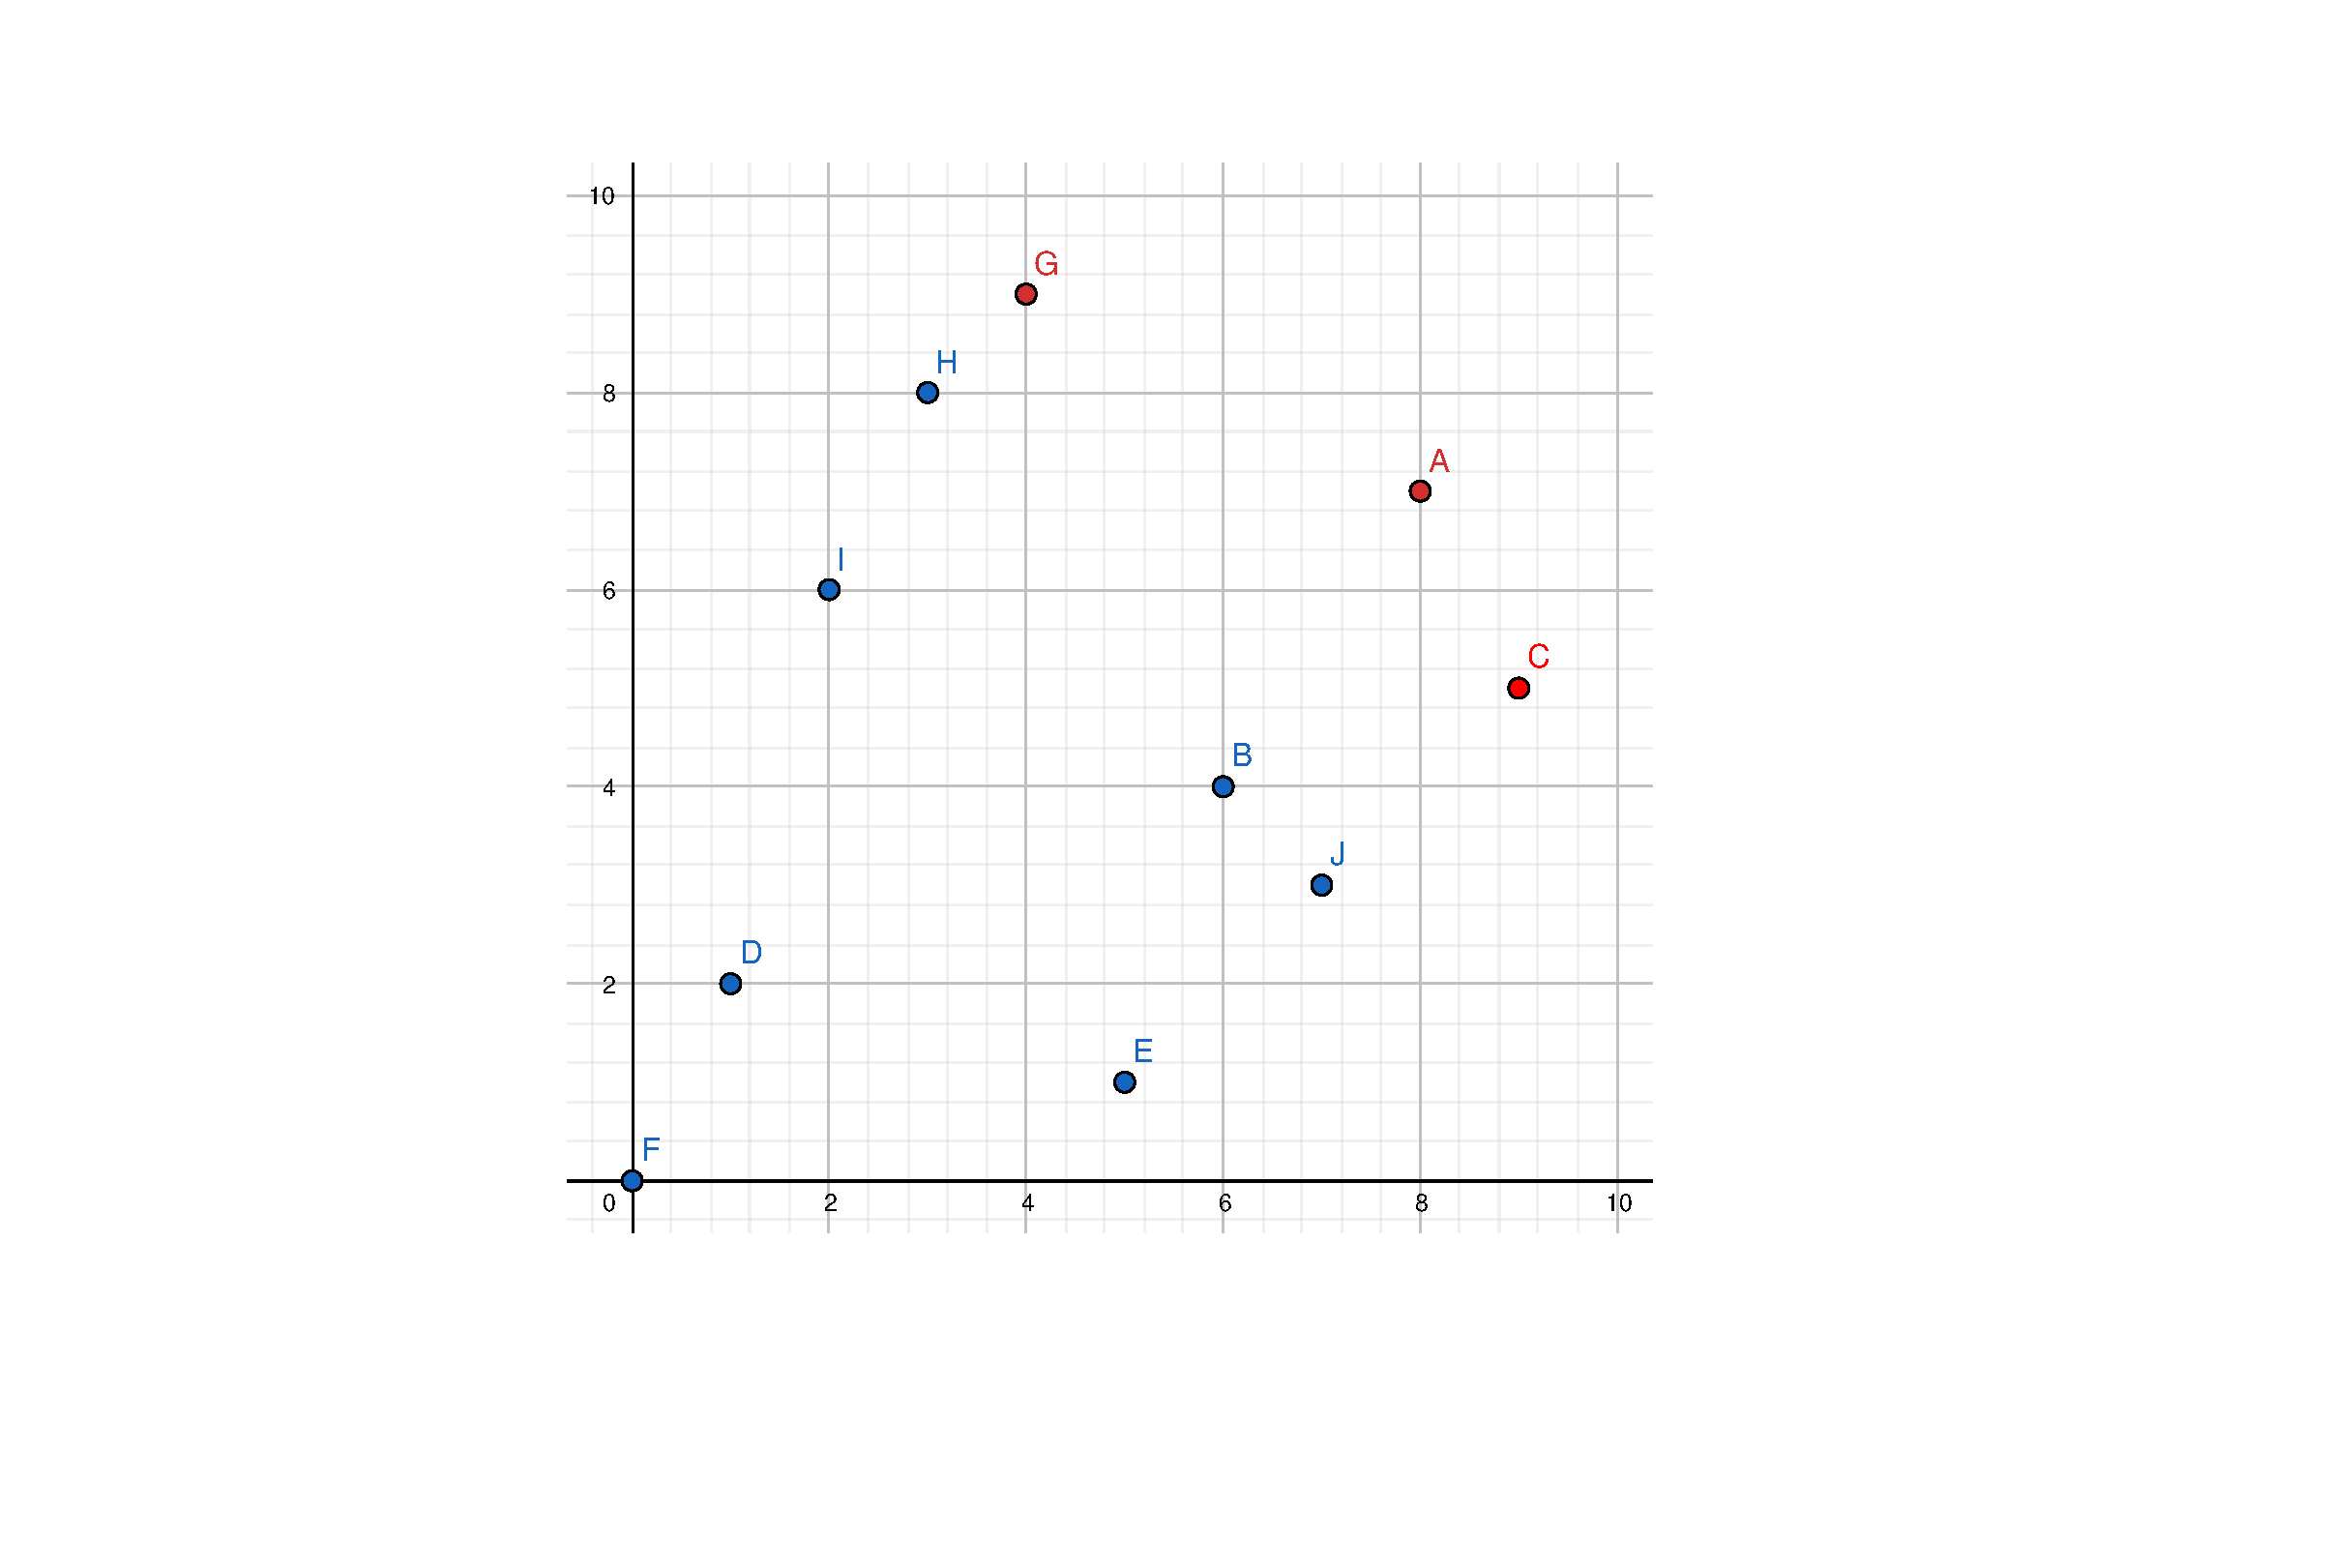
\includegraphics[scale=0.5]{算法设计作业7-3.pdf}
\end{wrapfigure}
\\
输入数据:\\
10\\
8 7\\
6 4\\
9 5\\
1 2\\
5 1\\
0 0\\
4 9\\
3 8\\
2 6\\
7 3\\
输出结果:\\
9 5\\
8 7\\
4 9\\
红色节点表示maxima节点.
\subsubsection{数据生成代码}
\begin{cppcode}
int x[1000000], y[1000000];
int main() {  // 7-3随机生成数据
    srand(time(NULL));
    freopen("7-3.in", "w", stdout);
    int n = 10;  // 总点数目,生成点范围在[0,...,n), [0,...,n)中间,保证两两之间横纵坐标不同
    cout << n << '\n';
    for (int i = 0; i < n; i++) x[i] = y[i] = i;
    random_shuffle(x, x + n);
    random_shuffle(y, y + n);
    for (int i = 0; i < n; i++) cout << x[i] << ' ' << y[i] << '\n';
    return 0;
}
\end{cppcode}
\section{问题四}
设有$a,b,c,d,e$五个整数和\cppinline{+,-,*,/}四个运算符. 对于任意给定的整数$n$,请设计一个算法,用给定的$5$个整数生成一个算术表达式(每个整数和每个运算符只能使用$1$次),使其运算结果等于$n$.
\subsection{问题分析}
考虑直接递归枚举所有可能的算术表达式形式,时间复杂度为$\O(5!4!)$,详细计算全部算术表达式总数为
\begin{equation*}
    5+(5\times 4)\times 4 + (5\times 4\times 3)\times(4\times 3) + (5\times 4\times 3\times 2)\times (4\times 3\times 2)+5\!\times 4\! = 6565
\end{equation*}
\subsection{算法分析}
直接使用递归枚举全部算术表达式的可能性,再使用逆波兰表达式计算每个算术表达式的结果,若与$n$相等则输出结果.
\begin{cppcode}
#include <iostream>
#include <stack>
#include <map>
using namespace std;

// use[][0]表示每个数是否使用过,uses[][1]表示每个符号是否用过
bool use[5][2];
// now[i]表示结果中第i位的值,i为偶数则是数字,反之为运算符
int now[9];
// 存储全部解
map<int, int> mp;

int n, a[5], rk[256];
int opt[] = {'+', '-', '*', '/'};
stack<string> ans;

void execute(stack<int> &stk, int opt) {
    int b = stk.top(); stk.pop();
    int a = stk.top(); stk.pop();
    if (opt == '+') stk.push(a+b);
    if (opt == '-') stk.push(a-b);
    if (opt == '*') stk.push(a*b);
    if (opt == '/') stk.push(a/b);
}

int calc(int x) {  // 利用逆波兰表达式求解当前计算式now[]的值
    stack<int> stk_num, stk_opt;
    for (int i = 0; i < x; i++) {
        if (i % 2 == 0) stk_num.push(now[i]);  // 数字
        else {  // 运算符
            while (!stk_opt.empty() && rk[now[i]] >= rk[stk_opt.top()]) {
                execute(stk_num, stk_opt.top());
                stk_opt.pop();
            }
            stk_opt.push(now[i]);
        }
    }
    while (!stk_opt.empty()) {
        execute(stk_num, stk_opt.top());
        stk_opt.pop();
    }
    mp[stk_num.top()]++;
    return stk_num.top();
}

string vec2str(int x) {  // 将now[]数组转化为字符串
    string ret = "";
    for (int i = 0; i < x; i++) {
        if (i % 2 == 0) ret += to_string(now[i]);
        else ret.push_back(now[i]);
    }
    return ret;
}

void dfs(int x) {  // x为当前枚举位置
    if (x % 2 == 1 && calc(x) == n) {
        string s = vec2str(x);
        ans.push(vec2str(x));
    }
    if (x == 9) return;  // 枚举到头了
    if (x % 2 == 0) {  // 偶数位为数字
        for (int i = 0; i < 5; i++) {
            if (use[i][0]) continue;
            use[i][0] = 1;
            now[x] = a[i];
            dfs(x+1);
            use[i][0] = 0;
        }
    } else {  // 奇数位为运算符
        for (int i = 0; i < 4; i++) {
            if (use[i][1]) continue;
            use[i][1] = 1;
            now[x] = opt[i];
            dfs(x+1);
            use[i][1] = 0;
        }
    }
}

int main() {
    rk['+'] = rk['-'] = 1;  // 设置优先级
    cin >> n;
    for (int i = 0; i < 5; i++) cin >> a[i];
    dfs(0);
    if (ans.size() == 0) cout << "No Solution" << '\n';
    cout << "Total Solution: " << ans.size() << '\n';
    while (!ans.empty()) cout << ans.top() << '\n', ans.pop();

    // 反向求出每个n对应的解的个数
    printf("\nn\tSolution Num\n");
    int tot = 0;
    for (auto i : mp) cout << i.first << '\t' << i.second << '\n', tot += i.second;
    cout << "Total expression: " << tot << '\n';
    return 0;
} 
\end{cppcode}
\subsection{测试结果与性能分析}
上述代码还能够输出该数值全部可能达到的结果,但由于篇幅过大这里就不进行演示,只展示与$n$相等的表达式结果:
\begin{cppcode}
Input:                  Input:                  Input:
151                     666                     5
1 2 3 10 100            3 10 20 33 97           3 10 20 33 97
Output:                 Output:                 Output:
Total Solution: 6       Total Solution: 8       Total Solution: 8
100/2*3+1               97/10-3+33*20           97/33+3
100*3/2+1               97/10-3+20*33           20/10+3
3*100/2+1               97/10+33*20-3           20*10/97+3
1+100/2*3               97/10+20*33-3           10*20/97+3
1+100*3/2               33*20-3+97/10           3+97/33
1+3*100/2               33*20+97/10-3           3+20/10
                        20*33-3+97/10           3+20*10/97
                        20*33+97/10-3           3+10*20/97

Input:                  Input:                  Input:
122                     -1036                   -101
3 10 20 33 97           3 10 20 33 97           3 10 20 33 97
Output:                 Output:                 Output:
Total Solution: 1       Total Solution: 1       Total Solution: 1
97/20*33-10             20-97/3*33              97-20/3*33
\end{cppcode}
\end{document}
